\documentclass[11pt]{article}


%----------------------------------------------------------------------------------------
%	Packages and configuration
%----------------------------------------------------------------------------------------

\usepackage[T1]{fontenc}
\usepackage{ucs} % Encoding errors
\usepackage[francais]{babel}
\usepackage{xltxtra} % More XELATEX
\usepackage{graphicx} % Permits to include some pictures
\usepackage{fontspec}
\usepackage{url} % Url links
\usepackage{float} % Adds options to floats like H
\usepackage[ocgcolorlinks]{hyperref}
\usepackage{fancyhdr}
\usepackage{metalogo}
\usepackage[titletoc]{appendix}
\usepackage{pdflscape} % Pour des pages au format paysage
\usepackage{enumitem}  % Pour pouvoir choisir le symbole de itemize : 
                       % \begin{itemize}[label={$\bullet$}]
\usepackage{tabu}
\usepackage{tabularx}
\usepackage{multirow}
\usepackage{lastpage}
\usepackage{longtable}
%\usepackage[left=3.5cm,right=3.5cm,top=2cm,bottom=2cm]{geometry} % Change margins

\hypersetup{colorlinks=true,allcolors=black}

\setmainfont{Sorts Mill Goudy}
\pagenumbering{arabic}
\urlstyle{same}
\tabulinesep =1mm
%----------------------------------------------------------------------------------------
%	Header
%----------------------------------------------------------------------------------------
\newcommand{\helv}{%
   \fontsize{9}{11}\selectfont}

   \lhead{\helv \parbox[b]{3.5cm}{ÉTS - Département de génie logiciel et des TI}}
   \chead{\helv \parbox[b]{7cm}{\centering LOG792 - Proposition - Optimisation des paramètres d’une éolienne en mouvement}}
\rhead{\helv \today \linebreak \thepage}
\lfoot{}
\cfoot{}
\rfoot{}

\setlength{\headwidth}{\textwidth}
\setlength{\headheight}{23pt}
% \setlength{\headheight}{1.2cm}
% \fancyhead[L]{
% \begin{tabularx}{\headwidth}{|cm{3.5cm}|X|l|}
% \hline
% \multirow{2}{*}{
\includegraphics[height=1cm]{images/ETS-noir-ecran-fond_transparent.png}} & \multirow{2}{3.5cm}{{\footnotesize Département de génie logiciel et des TI}} & 
% \mbox{\begin{tabularx}{\hsize}{l|l}
%       {\footnotesize Projet: LOG792}   & {\footnotesize \today} \\
%    \end{tabularx}} & {\footnotesize Version: 0.1}\\
% \cline{3-4}&& {{\footnotesize Titre: asdsad - Proposition asdsad sad asd }} & {\footnotesize Page \thepage \  de \pageref{LastPage}}
% \end{tabularx}\relax
% }

\renewcommand{\headrulewidth}{0.4pt}
%\renewcommand{\footrulewidth}{0.4pt}

%----------------------------------------------------------------------------------------
%	Document
%----------------------------------------------------------------------------------------

\begin{document}

\pagestyle{fancy}

\begin{titlepage}
\thispagestyle{fancy}

\newcommand{\HRule}{\rule{\linewidth}{0.5mm}} % Defines a new command for the horizontal lines, change thickness here

\center % Center everything on the page
 
%----------------------------------------------------------------------------------------
%	HEADING SECTIONS
%----------------------------------------------------------------------------------------

\textsc{\LARGE École de Technologie Supérieure}\\[1.5cm] % Name of your university/college

\vfill

\textsc{\Large Proposition}\\[0.5cm] % Major heading such as course name
\textsc{\large Projet de fin d'études \\ Département de génie logiciel et des TI}\\[0.5cm] % Minor heading such as course title

%----------------------------------------------------------------------------------------
%	TITLE SECTION
%----------------------------------------------------------------------------------------


\HRule \\[0.4cm]
{ \huge \bfseries Optimisation des paramètres d’une éolienne en mouvement}\\[0.4cm] % Title of your document
\HRule \\[1.5cm]
 
%----------------------------------------------------------------------------------------
%	AUTHOR SECTION
%----------------------------------------------------------------------------------------
\vfill

\begin{minipage}{0.4\textwidth}
\begin{flushleft} \large
\emph{Auteur:}\\
Pierre-Alexandre \textsc{St-Jean}\\
\small{<pa@stjean.me>}
\end{flushleft}
\end{minipage}
~
\begin{minipage}{0.4\textwidth}
\begin{flushright} \large
\emph{Superviseur:} \\
Dr. Christian \textsc{Desrosiers}\\
\small{<christian.desrosiers@etsmtl.ca>}
\end{flushright}
\end{minipage}\\[4cm]

% If you don't want a supervisor, uncomment the two lines below and remove the section above
%\Large \emph{Author:}\\
%John \textsc{Smith}\\[3cm] % Your name

%----------------------------------------------------------------------------------------
%	DATE SECTION
%----------------------------------------------------------------------------------------

\vfill

{\large \today}\\[3cm] % Date, change the \today to a set date if you want to be precise

%----------------------------------------------------------------------------------------
%	LOGO SECTION
%----------------------------------------------------------------------------------------

%\includegraphics{Logo}\\[1cm] % Include a department/university logo - this will require the graphicx package
 

\end{titlepage}

%----------------------------------------------------------------------------------------
%	DOCUMENT
%----------------------------------------------------------------------------------------

\vspace*{\fill}
\begin{center}
\section*{Résumé}
\addcontentsline{toc}{section}{Résumé}
\end{center}

Le club étudiant Chinook, afin de continuer son succès en compétition améliore constamment son éolienne. L'ajout d'un système mécanique et électronique de contrôle de l'angle d'attaque de celle-ci ainsi que du ratio de transmission permettra d'augmenter les performances du véhicule. Afin de commander ces nouveaux systèmes, un algorithme de contrôle doit être développé afin de gérer ces systèmes. Le présent projet propose donc de caractériser l'éolienne puis de créer un tel algorithme de contrôle de l'éolienne à l'aide des algorithmes génétiques.

\vspace*{\fill}
\clearpage


\section*{Table des matières}
\addcontentsline{toc}{section}{Table des matières}

\renewcommand{\contentsname}{Table des matières}
\makeatletter
\renewcommand{\tableofcontents}{\@starttoc{toc}%
}
\makeatother

\tableofcontents

\phantomsection

\listoffigures
\addcontentsline{toc}{section}{Table des figures}


\clearpage

\section{Problématique et contexte}

Le véhicule éolien Chinook\ref{fig:chinookHall} de l'ÉTS est un regroupement de personnes\footnote{\url{http://chinookets.com}} qui analysent, conçoivent et construisent un véhicule propulsée par une éolienne. Le véhicule participe, chaque année, depuis deux ans à une compétition de véhicules de ce type qu'ils ont remportés l'année dernière. Cette année le véhicule doit être améliorer afin de pouvoir rester compétitif. Pour ce faire un système électronique de controle de l'angle d'attaque des pales de l'éolienne sera installé. La transmission du véhicule sera aussi modifiée afin de pouvoir être contrôllée électroniquement. 

\begin{figure}[H]
  \centering
  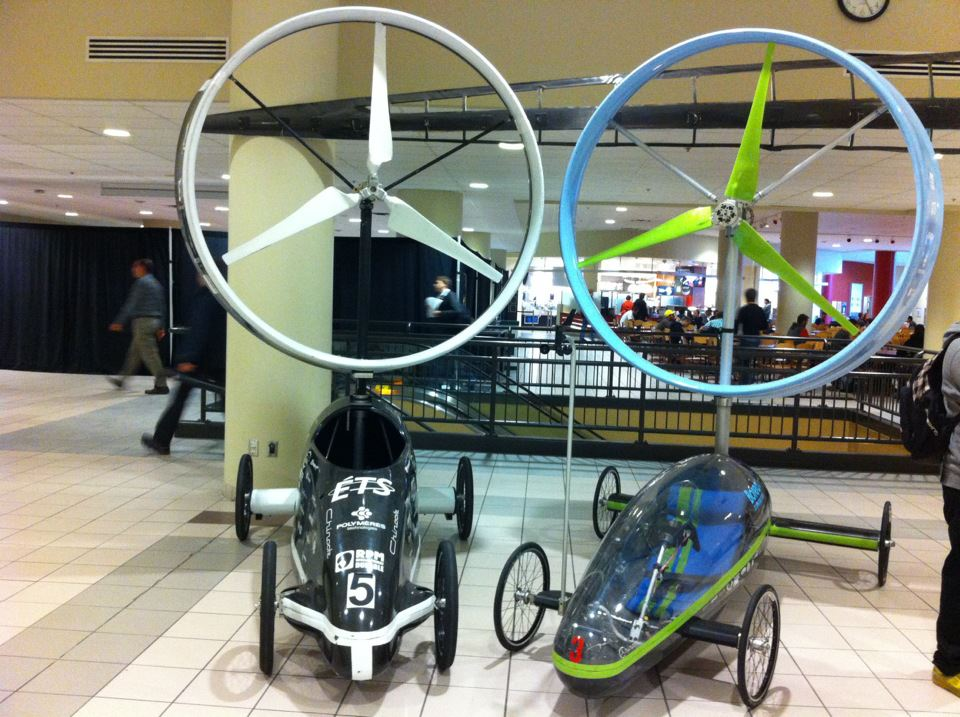
\includegraphics[width=0.5\textwidth]{images/chinook_1_et_2.jpg}
  \caption[Chinook 1 et 2]{Le Chinook 1 et le Chinook 2 en exposition dans le Hall A de l'ÉTS}
  \label{fig:chinookHall}
\end{figure}

Afin de pouvoir controller ces systèmes électroniques, des modèles de contrôle et d'optimisation de la puissance de l'éolienne doivent être créés. Les modèles théoriques applicables aux éoliennes standards doivent être modifiés afin de prendre en compte le fait que l'éolienne du Chinook est une éolienne mobile. Ainsi les systèmes de contrôles d'éoliennes fixes ne sont pas applicables dans le contexte d'une éolienne mobile.

\section{Objectifs du projet}

Le présent projet à pour but d'ammener l'éolienne du Chinook 3 [figure: \ref{fig:matRotor}] à opérer dans les conditions et à l'aide des paramètres d'opérations optimales. Pour ce faire, l'éolienne doit être caractérisé, un modèle de contrôle et d'optimisation de l'angle d'attaque ($\beta$) des pales et du ratio de transmission qui affecte la vitesse de rotation de l'éolienne ($\omega$) doit être conçu, analysé puis ce modèle doit être implanté dans le logiciel de la carte électronique de calcul.

Le système de contrôle pourra, à tout moment, changer l'angle d'attaque des pales ($\beta$) où le ratio transmission afin d'atteindre les performances optimales de l'éolienne dans les conditions de vitesse du véhicule et de vitesse du vent.


\begin{figure}[H]
  \centering
  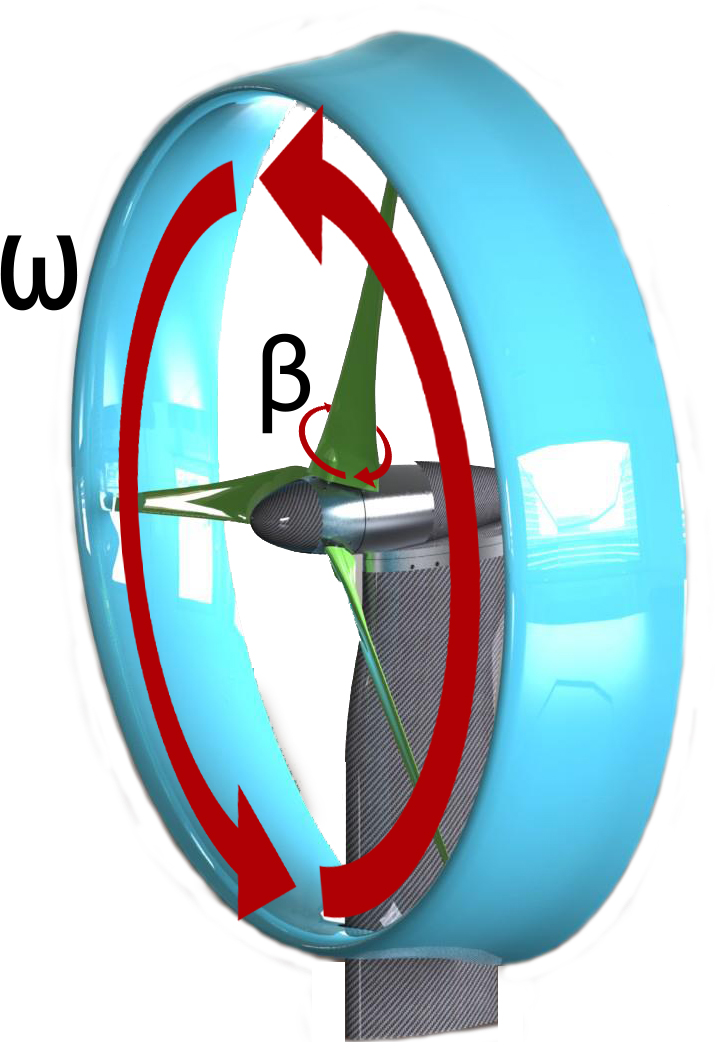
\includegraphics[width=0.5\textwidth]{images/matetrotorrotationnel.jpg}
  \caption[Mat et Rotor du Chinook 3]{Rendu 3D du mat et du rotor du Chinook 3}
  \label{fig:matRotor}
\end{figure}

Un tel modèle ainsi opérationnel dans les systèmes de contrôle du Chinook permettra au véhicule d'atteindre de meilleures vitesses et ce plus rapidement tout en permettant de conserver les vitesses atteintes et de mieux résister aux turbulences que par les années passées.

\section{Méthodologie}

La méthode utilisé dans ce projet sera adapté à partir de plusieurs méthode d'optimisation par algorithme génétique, entre autres celles provennant de \cite{GeneticField} et de \cite{Ouissam12}. Ces méthodes seront appliqués selon des processus de génie logiciel (développement dirigé par les spécifications, etc...). Tout au long du projet des pratiques provennant de méthodes agiles tel que Kanban\footnote{\url{https://en.wikipedia.org/wiki/Kanban_(development)}} et Scrumm\footnote{\url{https://en.wikipedia.org/wiki/Scrum_(development)}} 

Premièrement, le facteur de conversion de l'éolienne ($C_p$) doit être caractérisé. Pour ce faire on doit récupérer des données expérimentales de l'éolienne selon plusieurs paramètres puis on doit trouver une équation qui régit ces données. Afin de trouver l'équation, une régression de style "Curve-Fitting" tel que décrite dans \cite{GeneticField} à la section 12.2 sera utilisée.

Lorsque le comportement de l'éolienne sera caractérisé, un modèle mathématique de contrôle de l'éolienne sera généré à l'aide d'un algorithme génétique. La méthode décrite dans \cite{Ouissam12} sera améliorée et adaptée afin de convenir au contexte d'utilisation du Chinook et cette méthode sera utilisée afin de générer le modèle mathématique de contrôle.

Suite à la création de la formule de contrôle et à partir de l'architecture électrique et logiciel [Annexe \ref{sec:archELE}] du Chinook 3, on peut inclure ces équations à l'intérieur du Chinook dans la carte électronique de calcul [figure \ref{fig:carteElec}]. Les équations donneront en sortie: l'angle d'attaque et le ratio de transmission à appliquer. Ces données seront envoyés aux systèmes qui contrôlent les moteurs.

\begin{figure}[H]
  \centering
  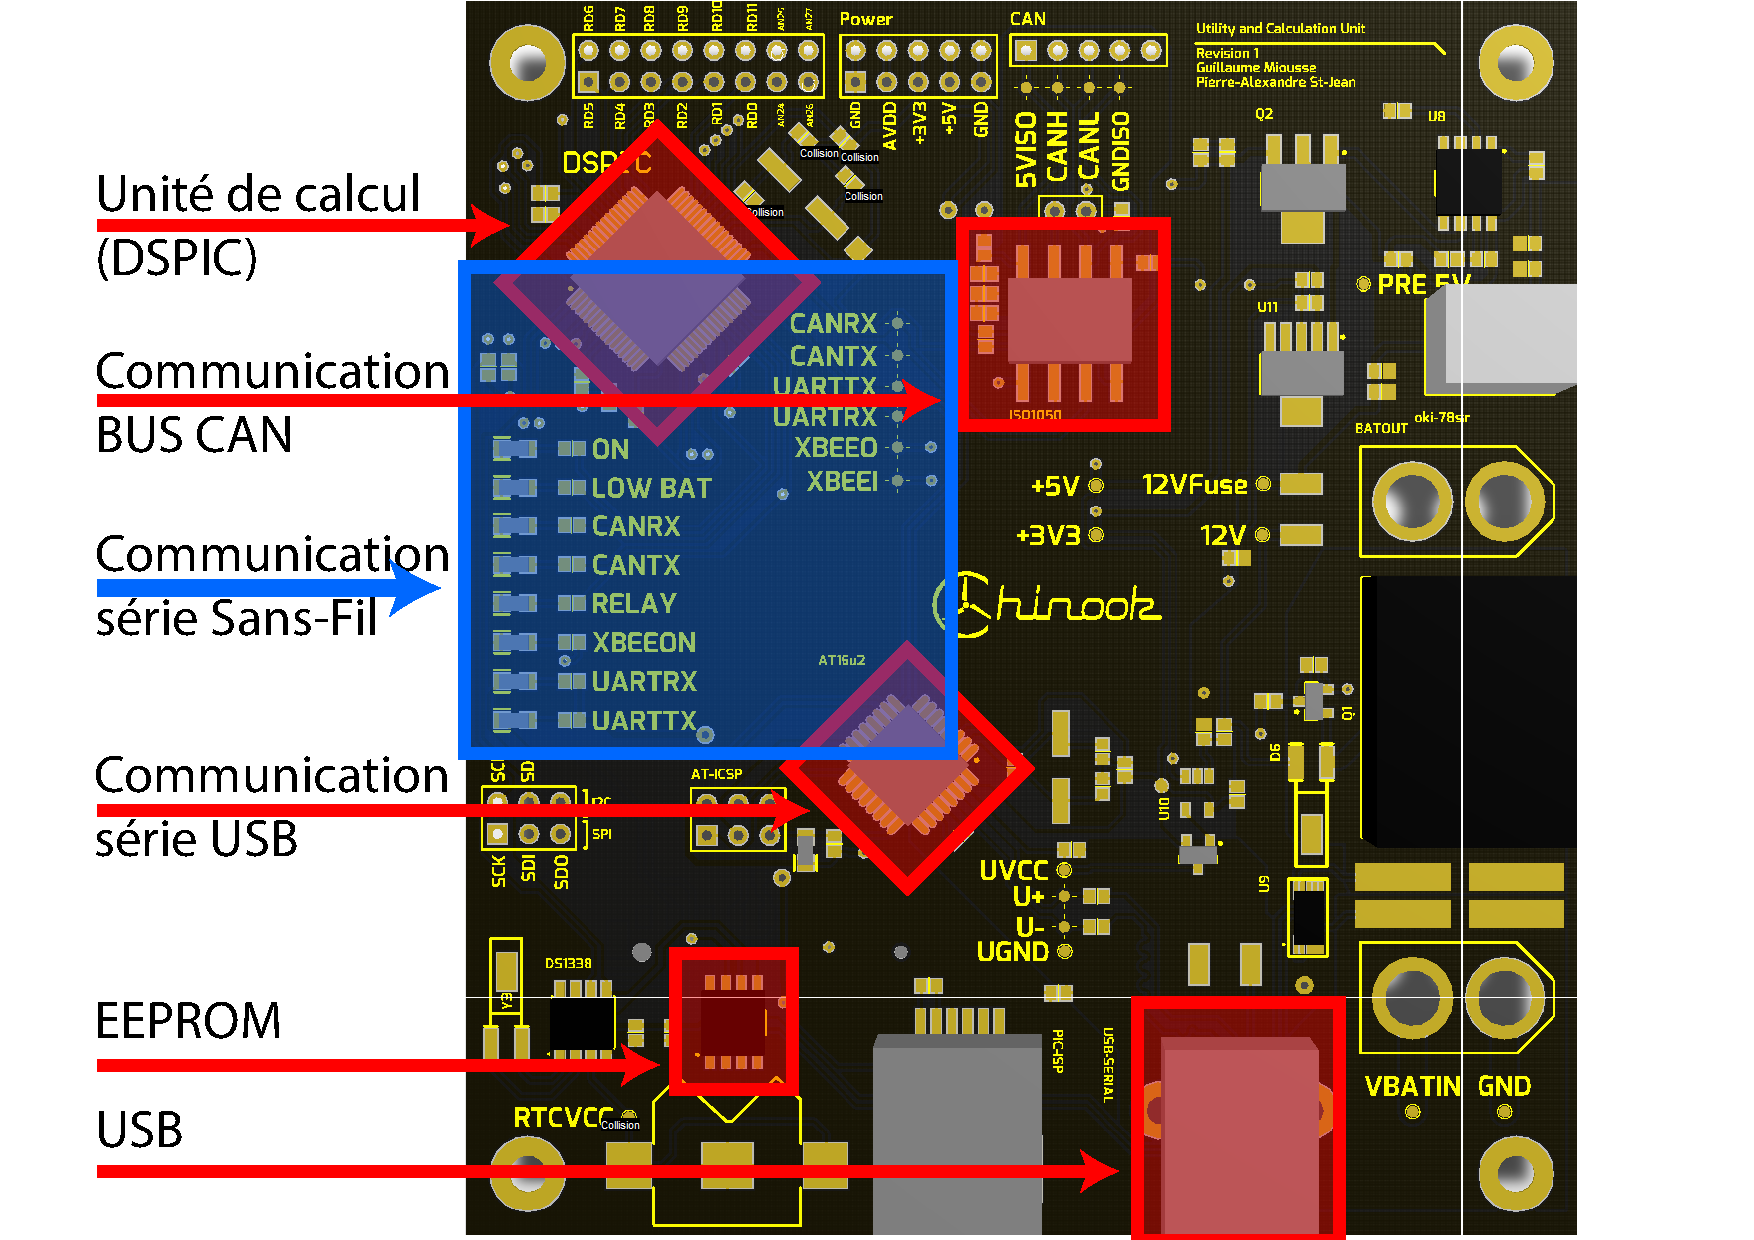
\includegraphics[width=0.7\textwidth]{images/3d-top-annoté.pdf}
  \caption[Carte électronique de calcul]{Carte électronique d'acquisition de données, de surveillance du courant électrique et de calcul de l'angle d'attaque des pales et du ratio de transmission}
  \label{fig:carteElec}
\end{figure}

Des tests sur route seront ensuite effectués avec le Chinook afin de valider si les modèles calculés à partir d'algorithmes génétiques fonctionnent.

Afin de permettre à l'éolienne de se comporter correctement lorsqu'elle est dans un autre état qu'en régime permanent, des états supplémentaires seront ajoutés à l'algorithme de contrôle, par exemple: lorsque la voiture va plus vite que l'éolienne (poussée) ou lorsqu'elle est à l'arrêt.


En résumé, le projet consiste en :
\begin{itemize}
  \item La récolte de données sur l'éolienne à différent $\beta$ et $\lambda$
  \item La caractérisation du facteur de conversion de puissance de l'éolienne ($C_p$), c'est à dire le ratio entre la puissance du vent fournie à l'éolienne et la puissance de sortie de celle-ci
  \item L'adaptation et l'amélioration de la méthode de \cite{Ouissam12} afin qu'elle convienne au contexte du Chinook. Cette méthode génere un modèle mathématique de contrôle de l'éolienne
  \item l'implémentation du modèle mathématique de contrôle de l'éolienne dans la carte électronique de calcul
  \item Les tests sur route afin de valider la méthode
\end{itemize}

\section{Livrables et planification}

\subsection{Description des atéfacts}

\begin{longtabu} to \linewidth {X[1,l]X[2,l]}
  Artéfact & Description \\ \hline
  Proposition de projet & Le présent document qui décris sommairement en quoi consistera le projet, ça planification et la façon dont il sera exécuté.\\ \hline
  Rapport d'étape & Document décrivant l'avancement du projet et la façon dont le projet est analyser et conçu \\ \hline
  Rapport final & Document décrivant le projet dans son ensemble.\\ \hline
  Présentation & Préparation et mise en page de la présentation du projet au département de Génie Logiciel et des TI à la fin de la session\\ \hline
  Article & Article scientifique décrivant la méthode utilisée pour caractériser l'éolienne et créer l'algorithme d'optimisation\\ \hline
  Spécifications & Documents de spécifications des différents sous-projets que ce projet génère.\\ \hline
  Carte électronique: implémentation de base & Implémentation permettant de faire fonctionner tout les composantes de la carte électronique et prêt à accueillir la fonction de calcul. Cet implémentation permet de faire fonctionner les modules de communication soit le XBEE, le module CAN et le module de USB-SERIAL. L'implémentation permettra aussi de faire fonctionner le module de mémoire morte (EEPROM), le module de surveillance électrique et le module d'horloge (realtime clock).\\ \hline
  Carte électronique: Logiciel d'optimisatione & Implémentation du logiciel d'optimisation génétique à l'intérieur de la carte électronique en language C\\ \hline
  Programme de caractérisation de l'éolienne & Programme d'algorithme génétique faisant une opération de Curve-fitting \\ \hline
  Outils de simulation & Outils mathématiques permettant de simuler le fonctionnement de l'éolienne dans des conditions réelles. \\ \hline
  Algorithme génétique d'optimisation & Algorithme permettant d'optimiser les paramètres de l'éolienne selon des conditions quasi réelles d'opération \\ \hline
  Données de banc d'essai & Données récoltés en fixant certains paramètres de l'éolienne. \\ \hline
  Algorithme génétique de caractérisation de l'éolienne & Algorithme permettant de caractérisé la fonction de puissance de l'éolienne en fonction des données récoltés \\ \hline 
  Outils de simulation \& de visualisation & Outils mathématiques et algorithmiques qui permettent de simuler des conditions fictive et de voir les performances de l'éolienne et des algorithmes selon ces conditions\\
  Planification de projet & La planification de projet initiale est produite à l'intérieur de ce document. Elle ensuite continuée sur la plateforme Trello (Voir la section \ref{sec:techoutils}) \\
   Environnement de développement & L'environnement de développement est l'ensemble des outils utilisés lors de ce projet. L'environnement de développement permet de bien intégrer les différents outils entre eux.
\end{longtabu}

\subsection{Planification}
\begin{tabu} to \linewidth {Xlll}
  \bfseries Tâche & Début - Fin & Effort estimé\\ \hline
  Fiche de renseignement  & 26 Mars 2013 & 1h \\
  Proposition de projet   & 6 Mai 2013 - 12 Mai 2013 & 15h \\
  Rapport Étape           & 12 Mai 2013 - 21 Juin 2013 & 25h\\
  Rapport Final           & 21 Juin 2013 - 31 Juillet 2013 & 30h\\
  Présentation            & 21 Juin 2013 - 31 Juillet 2013 & 5h \\
  Article                 & 12 Mai 2013 - 31 Juillet 2013  & 25h\\
  Planification du projet & 8 Mai 2013 - 31 Juillet 2013   & 5h\\
  Compétition Racing Aeolus 2013 & 17 Août & \\
  \hline
  Rencontre avec professeur superviseur & (Au besoin) & 3h\\
  \hline
  Mise en place de l'environnement de développement & 12 Mai - 18 Mai & 5h \\
  Spécification du projet & 12 Mai - 1 Juin & 15h \\
  \hline
  Programme de caractérisation de l'éolienne & 12 Mai - 30 Mai & 15h\\
  Récolte de données                         & Mi-juin & 12h \\
  Caractérisation de l'éolienne              & Mi-juin & 6h\\
  \hline
  Outils de simulation \& de visualisation   & 12 Mai & 15h \\
  Programme génétique d'optimisation         & 1 Juin - 15 Juillet & 30h \\
  \hline
  Carte électronique: implémentation de base    & 10 mars 2013 - 20 Mai 2013 & 30h \\
  Carte électronique: ajout du logiciel d'optimisation & 1 Juillet 2013 - 31 Juillet 2013 & 20h \\
  \hline
  Tests sur route & Mi-Juillet & 3 fois 6h \\
  \hline
\end{tabu}

\section{Risques}

\subsection{Risques et mitigation de ces risques}

\begin{table}[H]
  \begin{center}
\begin{tabu} to \linewidth {X[1.5,l]|X[3,l]}
  Risque & Description \& Mitigation \\ \hline
  Risque que la préparation du véhicule ne respecte pas les délais & Ce risque peut-être mitigé en ayant un bon suivi de l'avancement et de la construction du véhicule et en offrant de l'aide si nécéssaire. \\ \hline
  Complexité du domaine d'application & Le domaine de l'application des énegies éoliennes et de la mécanique des fluides est un domaine complexe, ce risque peut être mitigé en ayant les bons renseignements en main. Plusieurs ressources sont disponible, soit à l'intérieur du club étudiant Chinook ou auprès des professeurs spécialisés dans ce domaine.\\ \hline
  Manque de données & En s'assurant d'obtenir assez de données lors des sorties de banc d'essai, ce risque est facillement évitable.\\ \hline
  Non fonctionnement de la méthode d'optimisation & Ce risque peut être évité en se renseignant sur l'application et la pertinance de la méthode utilisée. Toutefois, la méthode manuelle de contrôle reste toujours disponible.\\ \hline
  Complexité du projet & Ce risque peut être évité en se documentant correctement sur les méthodes utilisés et en s'assurant de la compréhension de ces méthodes \\
\end{tabu}
  \end{center}
\end{table}

\subsection{Impact, probabilité et exposition aux risques}
\begin{table}[H]
  \begin{center}
    \begin{tabu} to \linewidth {X[3.5,l]|X[0.7,l]|X[1,l]|X[1,l]}
      Risque                              & Impact & Probabilité & Exposition \\ \hline
      Risque que la préparation du véhicule ne respecte pas les délais & Élevé & Élevé & 0.3734 \\
      Complexité du domaine d'application & Moyen & Haut   & 0.1698            \\
      Manque de données                   & Haut  & Faible & 0.0679            \\
      Non fonctionnement de la méthode d'optimisation & Haut & Faible & 0.0679 \\
      Complexité du projet                & Moyen & Bas    & 0.0309            \\
    \end{tabu}
  \end{center}
\end{table}


La façon de calculer l'impact des risques et leur probabilités est faite selon la méthode de PÉRIL\footnote{\url{http://msdn.microsoft.com/en-us/magazine/dd315417.aspx}}. Voir les tableaux en [Annexe \ref{annexePERIL}] afin de voir les calculs. 

\section{Techniques et Outils}

\begin{itemize}[label={$\bullet$}]
  \item Des pratiques de méthodes agiles et itératives provennant de Kanban, Scrumm et autres seront utilisées tout au long du projet.
  \item Les spécifications logiciel et du projet seront écrites à l'aide la de la méthode (Specification by example) décrite dans \cite{Adzic11}.

  \item Formattage des documents de remise à l'aide des logiciels libres \LaTeX et de \XeLaTeX et des nombreux paquetages disponibles (CTAN\footnote{\url{http://www.ctan.org/}}).

  \item Tout les documents et codes sources seront gérés avec le système de gestion de versions GIT\footnote{\url{http://git-scm.org}}.

  \item Le service de partage de fichiers Dropbox sera utilisé afin de partager plusieurs fichers entre différents postes et différentes personnes.

  \item Github\footnote{\url{https://github.com}} sera utilisé comme plateforme d'hôte et de collaboration de code source.

  \item Trello\footnote{\url{https://trello.com}} sera utilisé comme plateforme de gestion du projet. L'outil sera utiliser pour faire le suivi et la planification du projet.

  \item Mathematica sera utilisé
\end{itemize}

%\bibliographystyle{anotate}
\bibliographystyle{apalike}
%\bibliographystyle{plainnat}
%\bibliographystyle{development}
\bibliography{bibliography}
\addcontentsline{toc}{section}{Références}

\clearpage

%----------------------------------------------------------------------------------------
%	Annexes
%----------------------------------------------------------------------------------------
\section*{Annexes}
\addcontentsline{toc}{section}{Annexes}
\begin{appendices}


\section{Architecture Électrique du Chinook 3}
\label{sec:archELE}
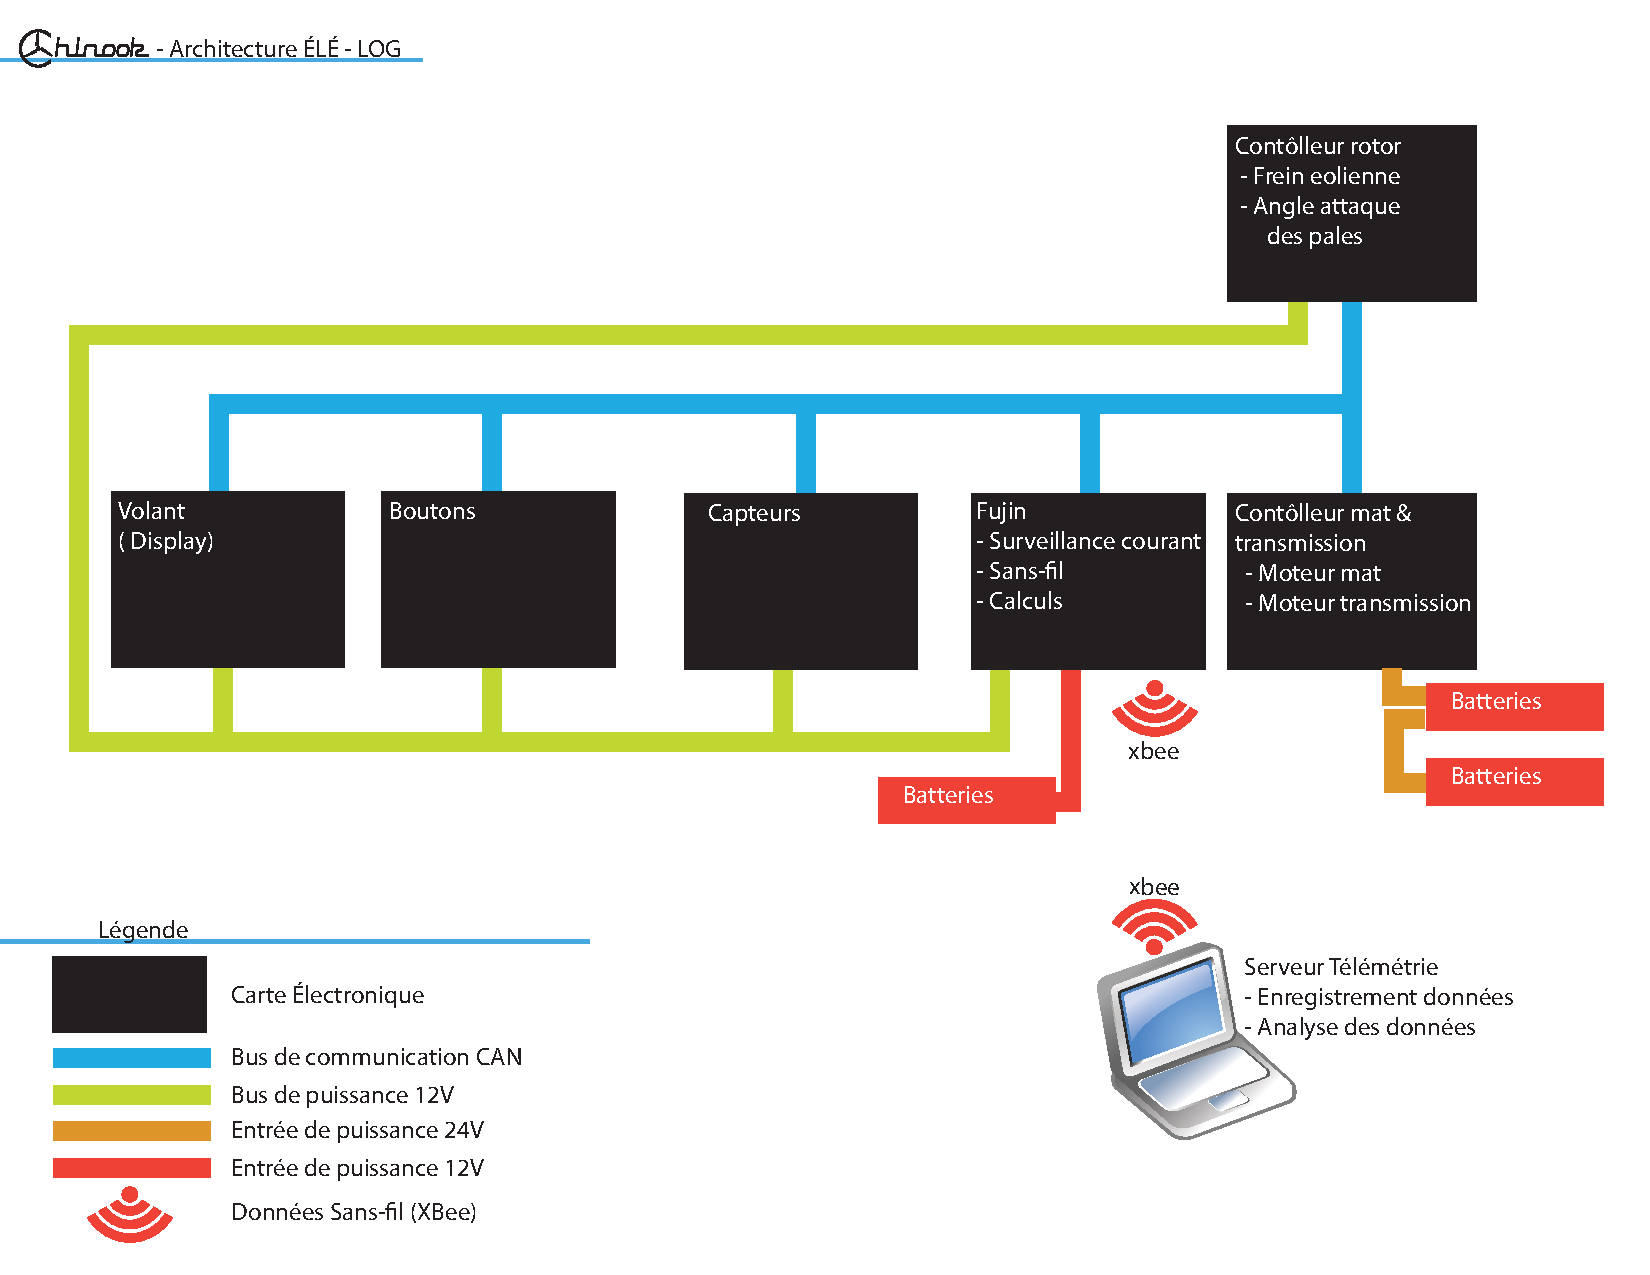
\includegraphics[height=1\textwidth,angle=90]{images/Architecture_ÉLÉ-LOG.pdf}

\clearpage
\section{Calcul de l'impact, la probabilité et de l'exposition aux risques}
\label{annexePERIL}
Voici les tableaux représentant le calcul de l'impact, la probabilité et l'exposition des risques selon la méthode de PERIL.

\subsection{Niveaux de probabilités/Impact}


\begin{tabu} to \linewidth {lX}
  Terme & Définition \\
  \hline
  Haut & Risque qui aurait une forte probabilité ou dont l'impact risquerait de mettre le bon bon déroulement du projet en jeu (retard de plusieurs jours) \\
  Moyen & Risque qui aurait une moyenne probabilité de survenir ou dont l'impact risquerait de retarder le projet de quelques jours.\\
  Bas & Risque qui aurait une faible probabilité de survenir ou dont l'impact risquerait de ne peu ou pas retarder le projet (quelques heures). 
\end{tabu}

\subsection{Calcul de Probabilité/Impact}

\begin{table}[H]
  \begin{center}
    \begin{tabu} to 0.5\linewidth {X[m]X[c,m]X[r,m]}
      Niveau & Calcul & Probabilité ou Impact \\
      \hline
      Haut  & \scalebox{1}{$\frac{1+ \frac{1}{2} +\frac{1}{3}}{3}$} & $0.6111$\\
      Moyen & $\frac{\frac{1}{2} +\frac{1}{3}}{3}$                  & $0.2777$\\
      Bas   & $\frac{\frac{1}{3}}{3}$                               & $0.1111$\\
    \end{tabu}
  \end{center}
\end{table}

\subsection{Exposition au risque}
L'exposition au risque est la probabilité multipliée par l'impact

\begin{table}[H]
  \begin{center}
    \begin{tabu} to 0.7\linewidth {X[1]|X[1]|X[1]|X[1]}
              & Haut     & Moyen    & Bas \\
      \hline
      Haut    & $0.3734$ & $0.1698$ & $0.0679$\\
      \hline
      Moyen   & $0.1698$ & $0.0712$ & $0.0309$\\
      \hline
      Bas     & $0.0679$ & $0.0309$ & $0.0123$\\
    \end{tabu}
  \end{center}
\end{table}


\end{appendices}

\end{document}
